
%%Copernicus Publications Manuscript Preparation Template for LaTeX Submissions
%% ---------------------------------
%% This template should be used for copernicus.cls
%% The class file and some style files are bundled in the Copernicus Latex Package, which can be downloaded from the different journal webpages.
%% For further assistance please contact Copernicus Publications at: production@copernicus.org
%% https://publications.copernicus.org/for_authors/manuscript_preparation.html


%% Please use the following documentclass and journal abbreviations for preprints and final revised papers.

%% 2-column papers and preprints
\documentclass[tc, manuscript]{copernicus}

\usepackage{makecell}
\usepackage{float}
\usepackage[section]{placeins}

\newcommand{\aref}[1]{\textbf{Reference #1}}
\newcommand{\afig}[1]{\textbf{Figure #1}}
\newcommand{\TODO}[1]{\textbf{TODO: \color{red}#1}}
\newcommand{\ian}[1]{{\textbf{\color{blue}Ian sayz:} \color{blue} #1} }
\newcommand{\mauro}[1]{{\textbf{\color{green}Mauro says:} \color{green} #1} }
\newcommand{\alpine}{\textit{ALPINE}\,}
\newcommand{\icesheet}{\textit{ICESHEET}\,}
\newcommand{\m}{$\,\mathrm{m}$\,}
\newcommand{\cm}{$\,\mathrm{cm}$\,}
\newcommand{\mma}{$\,\mathrm{mm  \, a^{-1}}$\,}
\newcommand{\mmma}{$\,\mathrm{m^3\, a^{-1}}$\,}
\newcommand{\mmms}{$\,\mathrm{m^3\, s^{-1}}$\,}
% \newcommand{\unit}[1]{$\mathrm{#1}$}

\begin{document}

\title{Subglacial and subaerial fluvial sediment transport capacity respond differently to water discharge variations}


\Author[1][IanArburua.Delaney@unil.ch]{Ian}{Delaney} %% correspondence author
\Author[1,2]{Andrew J.}{Tedstone}
\Author[3,4]{Mauro A.}{Werder}
\Author[3,4]{Daniel}{Farinotti}

\affil[1]{Institut des dynamiques de la surface terrestre (IDYST), Universit\'{e} de Lausanne, B\^{a}timent G\'{e}opolis, 1015 Lausanne, Switzerland}
\affil[2]{Department of Geosciences, University of Fribourg, Ch. du Musée 1700, Fribourg, Switzerland}
\affil[3]{Laboratory of Hydraulics, Hydrology and Glaciology (VAW), ETH-Z\"urich, H\"onggerbergring 26, 8093 Z\"urich, Switzerland}
\affil[4]{Swiss Federal Institute for Forest, Snow and Landscape Research (WSL) Z\"uricherstrasse 111, 8903 Birmensdorf, Switzerland}

\runningtitle{Subglacial sediment transport capacity}

\runningauthor{Delaney et al.}
\received{}
\pubdiscuss{} %% only important for two-stage journals
\revised{}
\accepted{}
\published{}

\firstpage{1}

\maketitle


\begin{abstract}
  Sediment transport capacity in both subaerial and subglacial channels depends on the shear stress exerted across the channel bottom.
  This quantity varies with water velocity and channel width.
  In subaerial channels,  sediment transport capacity can co-vary with water discharge because its variations are accommodated by changes in flow depth, width, and water velocity.
  By contrast, subglacial channels evolve at a slower rate than most water discharge variations, causing a variable relationship between channel shape, water velocity, and discharge.
  Using  sediment transport formulations and numerical models applied to two observed hydrographs, we evaluate the conditions where sediment transport capacity varies with water discharge in subglacial channels.
  Numerical experiments show that the changing channel size results in sediment transport capacity peaking before the maximum water discharge.
  This hysteresis in channel size causes a highly variable relationship between sediment and water discharge in a transport-limited subglacial system.
  The results also indicate that high subglacial sediment transport capacities can occur across a wide range of water discharges.
  We  then evaluate the conditions where subglacial sediment transport capacity is more variable than its subaerial counterpart.
  The numerical experiments of real hydrographs confirm that subglacial sediment transport is highly non-linear with respect to water discharge, creating more variability in sediment transport capacity.
  Yet,  formulations of subglacial sediment transport capacity show that it can covary with water discharge variations when subglacial channel size is in equilibrium. 
  The implications of these findings are discussed in the context of sediment discharge from glaciers with different hydro-climatic forcings.
  We also discuss the impact of different assumptions of channel behavior on sediment transport capacity.
  These findings can improve the interpretation of sediment discharge records in glacierized catchments.
\end{abstract}


\introduction  %% \introduction[modified heading if necessary]

Changes in glacier dynamics and hydrology have motivated numerous recent studies on sediment transport processes in cold regions \citep[e.g.][]{li2022,vergara2022,zhang2022}.
Increases in sediment transport have been observed in Greenland \citep{bendixen2017}, the European Alps \citep{costa2017}, the Himalayas \citep{li2021}, and the Andes \citep{vergara2022}.
To accurately explain observed changes in sediment transport in glacierized catchments, the processes controlling sediment discharge and its variations with water discharge need to be examined \citep[e.g.][]{riihimaki2005,swift2005}.

Glacier abrasion and quarrying sculpt landscapes, and create sediment that is transported fluvially over periods of millennia or longer \citep[c.f.][]{hallet1979,iverson2012,ugelvig2018}.
Pressurized subglacial water can transport this sediment from underneath glaciers \citep{walder1994,creyts2013,beaud2018,delaney2019} if it is reachable by the water.

In a transport-limited regime, sediment discharge is controlled by sediment transport capacity, which is defined as the amount of sediment the water can carry.
In both subglacial and subaerial channels, sediment transport capacity depends on the shear stress between water and the sediment it flows over \citep{shields1936,meyer1948,engelund1967}, along with the width of the channel bottom $w$ over which sediment mobilizes.
The shear stress $\tau$ responds to the velocity of water $v$ flowing through the channel so that
\begin{linenomath*}
  \begin{equation}
    \label{eq:tau}
    \tau \propto v^2.
  \end{equation}
\end{linenomath*}
% 
Following mass conservation, the mean velocity of the water flowing through a  channel is
\begin{linenomath*}
  \begin{equation}
    \label{eq:v}
    v = \frac{Q}{S},
  \end{equation}
\end{linenomath*}
where $Q$ is water discharge,  and $S$ is the channel's wetted area. 

In subaerial channels operating with open channel flow, $S$  evolves with changing water discharge $Q$, by changing both the channel width and the water depth \citep{leopold1953}.
The change in water depth results in a proportional increase in water velocity, and the shear stress $\tau$ increases according to Equation~\ref{eq:tau}.

The response of water velocity to changing water discharge in subglacial channels differs from subaerial ones, however.
The size of subglacial channels is controlled by the opposing processes of channel opening by frictional heating of water flow on the one hand, versus creep closure by ice flow on the other \citep{rothlisberger1972}.
As a result, the subglacial channel size only evolves relatively slowly over days, whereas water discharge can vary more quickly over hours \citep[e.g.][]{iken1986,andrews2014,nanni2020}.
Therefore, subglacial water flow behaves more like pipe flow over short periods (hours, days).
Changes in water discharge $Q$ are mainly accommodated by changing water velocity $v$ \citep[Equation~\ref{eq:v} and Figure~\ref{fig:cartoon}; ][]{alley1997}.

\begin{figure}[hbt!]
  \centering
  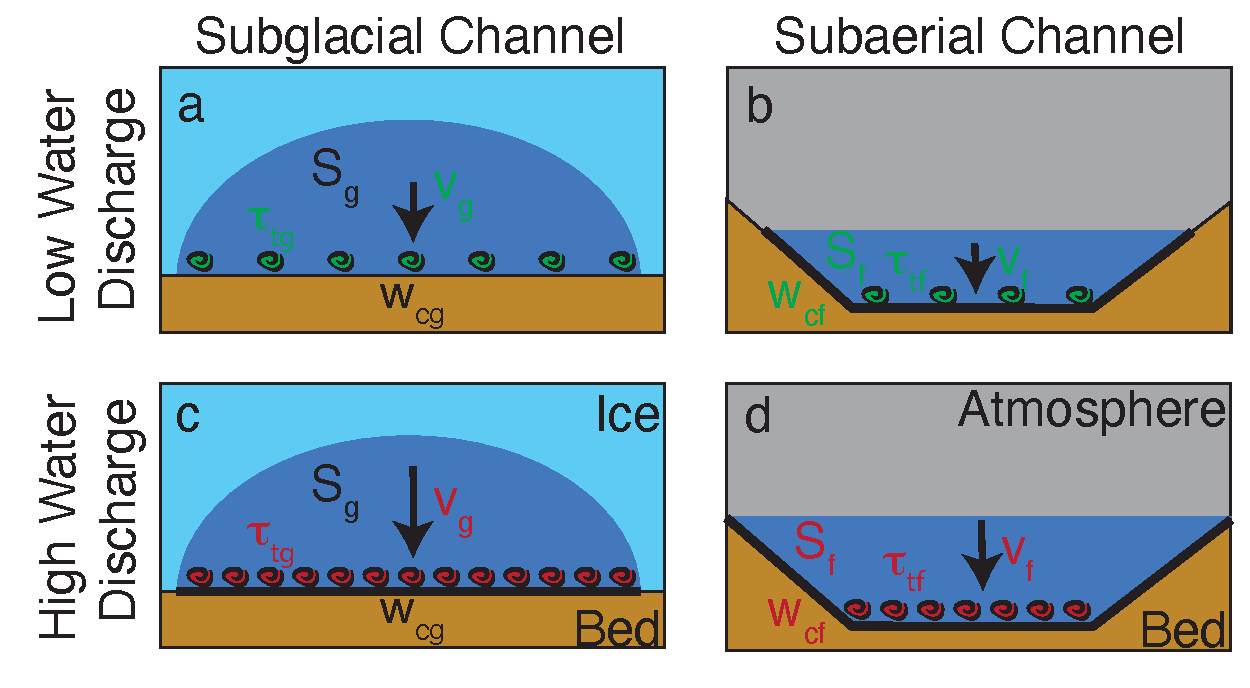
\includegraphics[width=0.8\linewidth]{Fig1.pdf}
  \caption{Sketch for the different responses of subglacial and subaerial channels to increased water discharge over short time scales.
    Arrow length denotes water velocity magnitudes in the subglacial (subaerial) $v_g$ ($v_f$) channels.
    $S_g$ ($S_f$) represents the wetted area in subglacial (subaerial) channels.
    The subglacial channel width $w_g$ remains unchanged, while the subaerial channel width $w_f$ evolves with water discharge.
    Subglacial (subaerial) shear stress $\tau_g$ ($\tau_f$) is responsible for the mobilization of sediment.
  }
  \label{fig:cartoon}
\end{figure}

Because of the above, sediment mobilization in subaerial and subglacial channels responds differently to changing water discharge.
These differences are implicitly included in a range of models quantifying sediment transport in both subglacial and subaerial channels  \citep[e.g.][]{walder1994,alley1997,tucker1997,creyts2013,beaud2018,delaney2019,hewitt2019,wickert2019}.
To date, several modeling frameworks examine subglacial sediment transport with evolving channel size \citep{creyts2013,beaud2018,delaney2019,hewitt2019}.
However, these works minimally discuss the impact of different hydrological regimes on sediment transport capacity underneath glaciers in the context of interpreting sediment transport records.
The few explicit parameterizations of subglacial sediment transport capacity with respect to water discharge assume fixed channel size  \citep{alley1997}. 
These formulations demonstrate a strongly non-linear response in subglacial sediment transport capacity to water discharge.
Yet, the continually evolving channels' size can impact variations in sediment transport capacity.
Understanding these processes is imperative for establishing the effect of hydro-climatic conditions on subglacial sediment dynamics,
especially as sediment discharge capacity controls the mobilization and deposition of sediment.
This makes it a fundamental aspect of subglacial sediment evacuation, especially over short timescales.

Despite the different physical processes between the subaerial and subglacial systems, observed water discharge and sediment export are often compared in contemporary glacierized catchments \citep[e.g.][]{willis1996,hodson1998,pearce2003,richards2003,swift2005,chu2009,tedstone2012,chu2012,overeem2017,delaney2018,swift2021,lu2022,andresen2024}.
Many of these studies discuss the disparity between water discharge and sediment export, especially given the role of sediment access or production.
Yet, a variable relationship between water discharge and sediment export could be expected from glaciers with evolving conduit size in a transport-limited regime, where sediment transport responds to the channel's hydraulic conditions, instead of sediment availability.
The response of sediment transport capacity to water discharge variations may affect the interpretation of sediment transport records in these glacierized catchments \citep[e.g.][]{ganti2016,mancini2023}.
This relationship must be clarified as sediment dynamics change in glacierized regions along with changing hydrology \citep[e.g.][]{brunner2019}, increasing variability of water discharge \citep{lane2019b} and occurrence of extreme glacier melt  \citep[e.g.][]{overeem2015,cremona2023} that may drive high magnitude sediment transport events.

This manuscript has two objectives: 1)  to establish whether sub-seasonal water discharge can co-vary with sediment transport capacity in subglacial systems, and 2) to evaluate the variability of  sediment transport capacity in subglacial channels with evolving channel size and different hydrographs compared to subaerial ones.
We use numerical models to examine sediment transport capacity in both subglacial channels that evolve in size and subaerial channels that remain fixed.
They are applied to proglacial hydrological records from an Alpine glacier in Switzerland (Fieschergletscher) and a land-terminating glacier in Greenland (Leverett Glacier).
Model outputs demonstrate the specific processes that can drive variability in sediment discharge capacity in subglacial systems.
We also run a model ensemble to evaluate the sediment transport capacity variability in subglacial channels compared to subaerial channels.
Lastly, we present algebraic formulations of the sediment transport capacity response to water discharge in subaerial, steady-state R-channel, and pipe flow conditions.
These formulations extend the relationships presented in \citet{alley1997} and illustrate the sediment transport capacity behavior of different channel assumptions.
Findings indicate differences in the relationships amongst water discharge, channel geometry, water velocity and sediment transport capacity in subglacial and subaerial channels.
The manuscript then discusses the implications of variability in sediment transport capacity from glaciers and the interpretation of sediment transport records.

\section{Study sites and data}
\label{sect:ss_data}

Water discharge data is from Alpine and ice sheet settings collected downstream of the glacier, and assumes no water storage in the proglacial area.
The Alpine site (labeled \alpine{}) is  Fieschergletscher in the Swiss Alps ($46^\circ\,29'\,07''$ N, $8^\circ\,08'\,3''$ E).
The water discharge data used here was collected at a $1$\unit{min} interval from May 24, 2014, to October 10, 2014 \citep[Figure~\ref{fig:Qw}\,a][]{felix2022}.

The Leverett Glacier in Greenland (labeled \icesheet{}) serves as the ice sheet setting.
Water discharge was measured roughly $2$\unit{km} downstream from the terminus ($67^\circ\,03'\,5''$ N, $50^\circ\,12'\,59''$ W), at a $5$\,\unit{min} time interval from May 28, 2012 to August 8, 2012 \citet[][Figure~\ref{fig:Qw}\,b]{tedstone2013}.


\begin{figure}[hbt!]
  \centering
  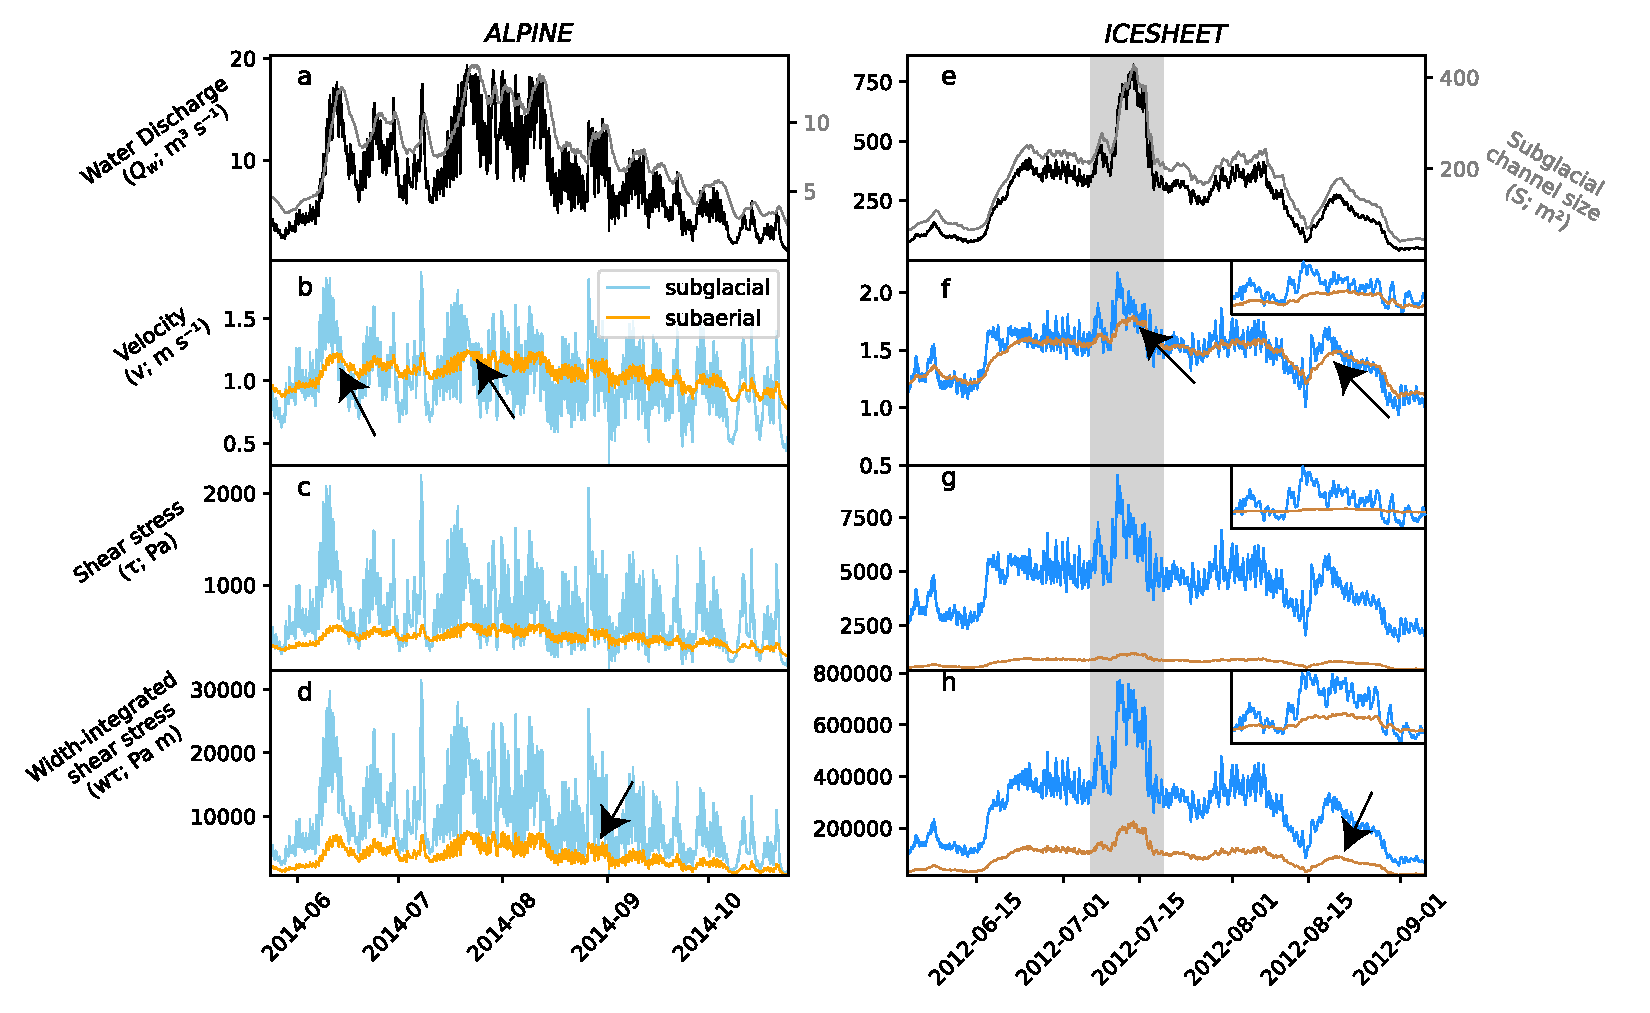
\includegraphics[width=0.9\linewidth]{Fig2.pdf}
  \caption{Water discharge from Fieschergletcher (\alpine) and Leverett Glacier (\icesheet).
    Note differences in variability and quantity of water discharge over the season.
  }
  \label{fig:Qw}
\end{figure}


\section{Methods}
\label{sect:meth}
The two models described below (Sections ~\ref{sect:sub_mode}~and~\ref{sect:fluv}) represent relationships amongst water discharge, water velocity, and channel geometry in both subaerial and subglacial channels (Table~\ref{table:vpm}).
Both models use the measured discharge to calculate water velocity, shear stress, and width-integrated shear stress, upon which both suspended sediment and bedload transport depend \citep[Figure \ref{fig:cartoon}; ][]{shields1936}.
Our choice to evaluate our results in terms of shear stress omits the selection of a sediment transport relationship and a grain-size parameter \citep[e.g.][]{shields1936,meyer1948}.


\subsection{Subglacial channel  model}
\label{sect:sub_mode}

The subglacial channel model accounts for the channel geometry and the water's velocity to evaluate the shear stress of water flowing across sediments underneath a glacier.
We use a lumped hydraulics model from \citet{werder2010b}, itself based upon  \citet{clarke1996}.

Here, it is assumed that the water is transported through a subglacial channel \citep[Figure~\ref{fig:cartoon}; ][]{rothlisberger1972} beneath a glacier with channel length $l$, with a flat bed and a mean thickness of $h_{ice}$.
The channel size grows from melt due to frictional heating from water flow and closes due to ice creep.
The formulation here does not consider the englacial storage of water.
The evolution of subglacial channel size $S_g$ is given as
\begin{linenomath*}
  \begin{equation}
    \label{eq:dS_dt}
    \frac{\partial S_g}{\partial t} = C_1 \frac{Q \Delta h}{l} - C_2 \left(h_{o}-\frac{\Delta h}{2}\right)^n\,S_g,
  \end{equation}
\end{linenomath*}
\noindent where $t$ is time, $C_1= (1-\rho_wc_pc_t)\,\frac{\rho_wg}{\rho_iL}$ and $C_2=2A(\frac{\rho_wg}{n})^n$ are constants (values in Table~\ref{table:vpm}), $g$ is the acceleration due to gravity, $Q$ is water discharge, $\Delta h$ is the hydraulic head drop change over $l$, $h_{o}= \frac{\rho_i}{\rho_w} h_{ice}$ is the mean ice overburden pressure expressed in meter water equivalent ($\rho_w$ is density of water; $\rho_i$ is density of ice), and $n$ is Glen's n \citep[usually $n=3$; ][]{glen1955}.
The first term on the equation's right side represents the channel opening by frictional heating, while the following term represents channel closure from ice deformation.


Following the Darcy-Weisbach equation, the head drop $\Delta h$ is
\begin{linenomath*}
  \begin{equation}
    \label{eq:dh}
    \Delta h \,  = l \,\frac{1}{2g} \,f_i\,\frac{v_{g}^{2}}{D_h},
  \end{equation}
\end{linenomath*}
\noindent where $f_r$ is a friction factor, $D_h$ is the hydraulic diameter, $l$ is the channel length, and $v_g=\frac{Q}{S_g}$ is the water velocity.
% 
The hydraulic diameter $D_h$ is converted to wetted area $S_g$ with
\begin{equation}
  \label{eq:Dh2S}
  S_g= \frac{D_h^2}{2}\,\frac{(\frac{\beta}{2}+\sin \frac{\beta}{2})^2}{\beta - \sin \beta},
\end{equation}
where $\beta$ is the central angle of the circular segment that comprises the channel (the Hooke angle, \citet{hooke1990}). $\beta =\pi$ corresponds to a semi-circular channel and smaller values of $\beta$ result in shallow, wide channels.
This completes the subglacial hydraulic model which is described by the state variables $S_g$ and $\Delta h$.

The shear stress, $\tau_g$, between the water and the channel bed results from the Darcy-Weisbach formulation
\begin{equation}
  \label{eq:tau_g}
  \tau_g=\frac{1}{8}\,f_r\,\rho_w\,v_g^2,
\end{equation}
% 
where $v_g = \frac{Q}{S_g}$ is the water velocity.
% 
The width of the channel floor $w_g$ is represented as
\begin{equation}
  \label{eq:dh2wc}
  w_g = 2  \sin \frac{\beta}{2} \sqrt{\frac{2\, S_g}{\beta -\sin \beta}}.
\end{equation}
% 
This value establishes the integrated shear stress across the channel $w_g\tau_g$.

\subsection{Subaerial channel  model}
\label{sect:fluv}

The hydraulics parameterization presented in \citet{tucker1997} is implemented to represent the subaerial channel.
This model uses mass conservation and the Darcy-Weisbach relationship and assumes that the channel is sufficiently wide compared to its depth.
This latter assumption means that the hydraulic radius is well approximated by the flow depth.
Therefore, the resulting shear stress $\tau_f$ at the river bed is
\begin{linenomath*}
  \begin{equation}
    \label{eq:DW_tau}
    \tau_f=\frac{\rho_w\,g^{\frac{2}{3}}\,f_f^{\frac{1}{3}}}{2}\, \Big(\frac{Q}{w_f} \Big)^{\frac{2}{3}} \,\nabla z_c^{\frac{2}{3}},
  \end{equation}
\end{linenomath*}
where $\nabla z_c$ is the channel slope, and $f_f$ is the friction factor for subaerial channels \citep{tucker1997}.
Channel width $w_f$ is
\begin{equation}
  \label{eq:wcf}
  w_f = k \, Q^{\alpha},
\end{equation}
% 
where $k$ is a constant and $\alpha=\frac{1}{3}$ is a commonly chosen exponent \citep{leopold1953}.
Also following the Darcy-Weisbach, subaerial water velocity, $v_f$, is given as
\begin{equation}
  \label{eq:vf}
  v_f = \sqrt{\frac{8\,\tau_f}{f_f\,\rho_w}}.
\end{equation}
% 
As mentioned above, the width-integrated shear stress is $w_f\tau_f$.

Note that this subaerial channel model is purely algebraic, whereas the subglacial model comprises a differential equation for the evolution of $S_g$.
Thus, the channel size in the subaerial model has no history dependence on the discharge $Q_w$, whereas the subglacial one does (Equation~\ref{eq:dS_dt}).

\begin{table}[hbt!]
  \centering
  \caption{Variables, parameters, and constants used in this work.
    Where two values are given, the first refers to  \alpine{}, a scenario from Fieschergletscher, and the second to a glacier marginal to the \icesheet{} a scenario from Leverett Glacier.
    A second line refers to the range of values examined in the parameter search.}
  \small 
  \begin{tabular}{ l  c  c c }
    Name &Symbol&  Value&Units \\
         && (\alpine{} or \icesheet{})\\
    \hline
    \textbf{Variables}  & & & \\
    Water discharge  & $Q$& & $\mathrm{m^{3}\,s^{-1}}$ \\
    Water velocity (subglacial, subaerial)  & $v$, ($v_g,\,v_{f}$)& & $\mathrm{m\,s^{-1}}$ \\
    Channel wetted area (subglacial, subaerial) &  $S_g, S_f$& & $\mathrm{m^2}$     \\
    Channel depth (subaerial) & $H$&& $\mathrm{m}$\\
    Hydraulic diameter &$D_h$&&$\mathrm{m}$\\
    Width of channel floor (subglacial, subaerial) & $w$, ($w_g,w_f$)&  & $\mathrm{m}$     \\
    Hydraulic head &$\Delta h$&& $\mathrm{m}$\\
    Hydraulic gradient &$\Psi=\frac{\Delta h}{l}$&& $\mathrm{m\, m^{-1}}$\\
    Shear stress (subglacial, subaerial) & $\tau$, ($\tau_g,\,\tau_f$) && $\mathrm{Pa \, m^{-2}}$ \\
    Stream power & $\Omega$ && $\mathrm{ kg \, m\, s^{-3}}$ \\


    \textbf{Parameters and Constants}  & & &\\
    Gravitational constant&$g$& $9.81$&$\mathrm{m\,s^{-2}}$\\
    Density of water & $\rho_w$& $1000$ & $\mathrm{kg\,m^{-3}}$ \\
    Density of ice & $\rho_i$& $900$ & $\mathrm{kg\,m^{-3}}$ \\
    Hooke angle of channel & $\beta$ & $\frac{\pi}{6}$ & \unit{rad}\\
         && ($\frac{\pi}{10}$, $\pi$) & \\
    Friction factor (subglacial, subaerial) & $f$, ($f_r$, $f_f$) & -($5$, ($16$, $3$)) & $\mathrm{(-)}$ \\
         && ($0.01$, $21$) & \\
    Glacier thickness &$h_{ice}$& $225$ or $740$  &\unit{m}\\
    Effective glacier thickness &$h_o$&$\frac{\rho_i}{\rho_w} h_{ice}$  &\unit{m}\\
    Effective glacier length &$l$& $7,000$ or $26,000$&\unit{m}\\
    Constant $1$ in Equation~3 &$C_1$&$2.2\times10^{-5}$&\unit{m}$^{-1}$\\
    Constant $2$ in Equation~3 &$C_2$&$3.7\times10^{-13}$&\unit{m}$^{-n}\,s^{-1}$\\
    Latent heat of fusion &$L$&$333.5 $&\unit{kJ\,kg}$^{-1}$\\
    Pressure melting coefficient &$c_t$&$7.5\times 10^{-8}$&\unit{K\,Pa}$^{-1}$\\
    Specific heat capacity of water &$c_p$&$4180$&\unit{J\,kg}$^{-1}$\unit{K}$^{-1}$\\
    Ice flow constant &$A$& $5.3\times10^{-24}$ &\unit{Pa}$^{-n}$\,$s^{-1}$\\
    Ice flow exponent &$n$& $3$ &$\mathrm{(-)}$\\
    
    Gradient of channel bed (subaerial) &$\nabla z_c$ &$0.02$& $\mathrm{(-)}$\\
         &&($.01$, $0.05$) & \\
    Subaerial channel factor & $k$ &$8$ & $\mathrm{s\,m^{-2}}$\\
    Channel geometry exponent &$\alpha$&$\frac{1}{3}$ &$\mathrm{(-)}$ \\
         &&($\frac{1}{3}$, $\frac{1}{2}$) & \\
    \hline
  \end{tabular}
  \label{table:vpm}
\end{table}

\FloatBarrier
\subsection{Implementation}
\label{sect:imp}

The models above are applied to proglacial discharge records from the Fieschergletscher (scenario \alpine{}) and the Leverett Glacier (scenario \icesheet{}).
The model outputs represent generalizable sediment transport characteristics from these hydrographs, rather than actual hydraulic conditions.
To generalize these scenarios, \alpine{}  is exemplified by relatively thin ice thickness \citep[$h_{ice}$= $225$\,\unit{m}][]{grab2021}, low water discharge ($\sim\,10$\,\unit{m}$^3$\,\unit{s}$^{-1}$) and high diurnal variability in water discharge at Fieschergletscher (Figure~\ref{fig:Qw}\, b).
\icesheet{}  is exemplified by thick ice  \citep[$h_{ice}$= $700$\,\unit{m}; ][]{morlighem2017}, high water discharge ($\sim\,300$\,\unit{m}$^3$\,\unit{s}$^{-1}$)  and low diurnal variability in water discharge at Leverett glacier (Figure~\ref{fig:Qw}\, b).

In the first experiment, the models are applied to a reference test case for each glacier.
These experiments assumes  a subglacial channel with $\beta=\frac{\pi}{6}$ and a subaerial channel with $\alpha = \frac{1}{3}$ and slope of $0.02$ (Table~\ref{table:vpm}).
Both friction factors $f_r$ and $f_f$ are tuned so that reasonable water velocities \citep[$\sim\,1- 1.5\,$\unit{m}\,\unit{s}$^{-1}$][]{werder2010b,chandler2013} occur for both \alpine{} and \icesheet{}.
To test the covariance between sediment transport capacity and water discharge, model outputs are compared to water discharge from the glaciers using Spearman rank correlation.
This metric accounts for the ordering of values, but not their magnitude.
Rank correlation reduces the impact of the non-linear relationship between sediment transport capacity and hydrology.


The second experiment aims to characterize the variability in sediment discharge capacity in subglacial relative to subaerial channels across a range of channel slopes and shapes, and friction factors.
Additionally, we examine the effects of differing water discharge smoothing periods from $15$\,\unit{min} up to $15$\,\unit{days}.
The results below present water velocity ($v_g$, $v_f$), shear stress ($\tau_g$, $\tau_f$), and width-integrated shear stress ($w_g\tau_g$, $w_f\tau_f$) from the subglacial and subaerial models.
For brevity, these values together are referred to as ``model outputs'' in the text.
To evaluate variability, we subtract the model outputs from their daily averages. 
This creates a time series that is detrended from the seasonal variations in the model outputs and has an approximately normal distribution.
We then present the variability in the model output by taking the standard deviation of this detrended time series.

The effects of channel shape, gradient, and roughness are established by running the model with random parameter values of channel slope and geometry factors ($\beta$,$\nabla z_c$, and $\alpha$) and friction factors ($f_r$ and $f_f$; see Table~\ref{table:vpm} for value range).
Runs with parameter combinations are accepted if their mean subglacial water velocity over the season lies between $0.5$\,\unit{m}\,\unit{s}$^{-1}$ and $2$\,\unit{m}\,\unit{s}$^{-1}$ or if subaerial water velocity lies between $0.3$\,\unit{m}\,\unit{s}$^{-1}$ and $1.2$\,\unit{m}\,\unit{s}$^{-1}$ \citep[e.g.][]{werder2010b,magnusson2012,chandler2013}.
To be accepted, subglacial model runs must experience a flotation fraction ($\frac{\Delta h}{2\,h_o}$) of above $1.2$ for less than $2.5$\,\% of the run.
A model spinup dictates the initial condition of cross-sectional area $S_g$.
The spinup consists of applying the maximum observed water discharge of the first $4$ days of the study period to the model until there is no change in the channel area $S_g$. 

The routine runs until $100$ different parameter combinations for each water discharge smoothing period are accepted with the conditions described above.
To test the effects of variability in water discharge, it is averaged over the smoothing period ranging 



\section{Results}

\FloatBarrier

\subsection{Changing subglacial channel size drives different timing and variability in sediment transport capacity}

The first numerical experiment aims to quantify the sources of increased variability in the subglacial model outputs as they exhibit different seasonal evolutions and peaks (Figure~\ref{fig:model_outs}).
Variable relationships between model outputs and water discharge emerge for the subaerial and subglacial cases due to the hysteresis in channel size in the subglacial model (Equation~\ref{eq:dS_dt}).
Because subaerial channels have no history dependence, each water discharge value in the subaerial channel produces a unique water velocity, shear stress, and width-integrated shear stress (Section~\ref{sect:sub_mode}).
This characteristic results in a perfect rank correlation between the variables and water discharge (Figure~\ref{fig:Qw_vari}).
An inconsistent relationship between subglacial model outputs and water discharge persists across the range of parameters examined in the ensemble runs (see Section~\ref{sect:ensemble}; Figure S15).
\begin{figure}[hbt!]
  \centering
  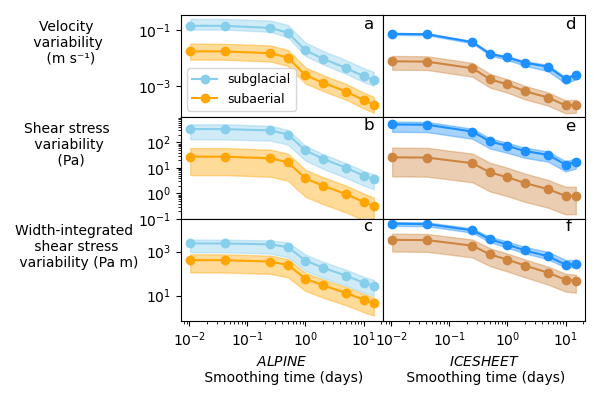
\includegraphics[width=\linewidth]{Fig5.png}
  \caption{Model outputs from simulations using the hydrographs in panels a and e for the scenarios \alpine{} (a-d) and \icesheet{} (e-h).
    Black (gray) lines in a and e represent the subglacial channel size (water discharge).
    Blue (orange) lines represent outputs from the subglacial (subaerial) channel.
    Data are shown at $15$\unit{min} intervals.
    Arrows show examples where variables peak in the subglacial channel before the subaerial one.
    Insets in f-h show the peak melt event denoted by the shaded area in panels e--h, with an arbitrary y-axis.
  }
  \label{fig:model_outs}
\end{figure}

Peaks in subaerial model outputs occur coincident with peaks in water discharge (Figure~\ref{fig:model_outs}).
In the subglacial channel, peaks in model outputs generally occur when water discharge increases at the fastest rate, but before the maximum water discharge.
Reduced water velocity takes place when water discharge stabilizes at its peak and channel growth continues.
As a result, subglacial sediment transport capacity is greatest on the hydrograph's rising limb, relative to the falling limb. 

The history dependence on channel size in subglacial channels means that different sediment transport characteristics, such as velocity, occur across a large range of water discharges.
For instance, in subglacial channels in \alpine{},  high water velocity values and shear stresses can occur from a low water discharge  ($\sim\,4$\,\unit{m}$^3$\,\unit{s}$^{-1}$) to the maximum water discharge at over $17$ \,\unit{m}$^3$\,\unit{s}$^{-1}$ (Figure~\ref{fig:Qw_vari}\,a).
In \icesheet{}, water velocities close to the seasonal mean value can occur at water discharges between roughly $150$ \,\unit{m}$^3$\,\unit{s}$^{-1}$ and $310$ \,\unit{m}$^3$\,\unit{s}$^{-1}$.
The subglacial channel's evolving width can counteract some of these effects.
Width-integrated shear stress generally increases with water discharge, with greater rank correlation compared to water velocity or shear stress (\alpine{}, Figure~\ref{fig:Qw_vari} a--c).
Yet, even the width-integrated shear stress can vary substantially relative to water discharge.
The highest values of width-integrated shear stress occur at water discharge values ranging from roughly $11$ \,\unit{m}$^3$\,\unit{s}$^{-1}$ to over $17$ \,\unit{m}$^3$\,\unit{s}$^{-1}$.
The variability in width-integrated shear stress is less pronounced in the \icesheet{} scenario, where the hydrograph has less diurnal variability (Figure~\ref{fig:Qw_vari} c, f).
This results from the discharge variations being in closer equilibrium with subglacial channels compared to \alpine{} (Sections~\ref{sect:scaling} and~\ref{sect:ensemble}).

\begin{figure}[hbt!]
  \centering
  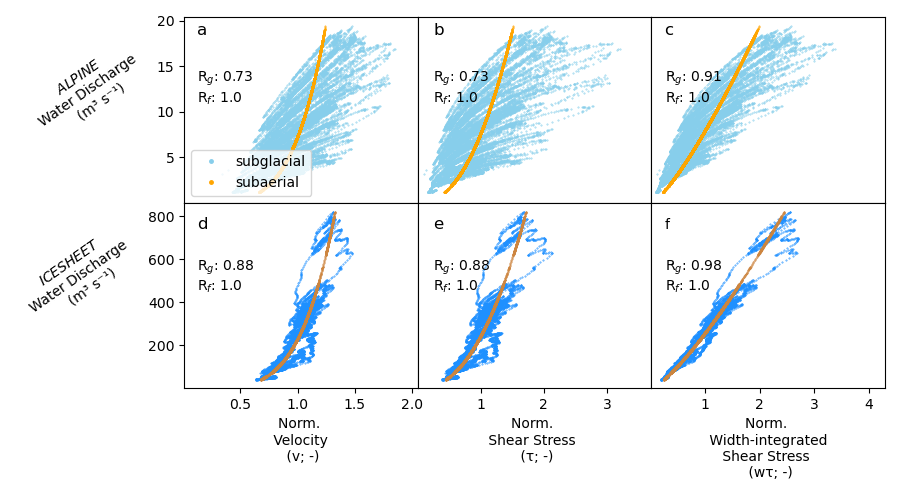
\includegraphics[width=0.8\linewidth]{Fig6.png}
  \caption{
    Relationship between water discharge and normalized velocity, shear stress, and width-integrated shear stress for \alpine{} (a-c) and \icesheet{} (d-f).
    Variables on the x-axis have been normalized to mean values.
    $R_g$ ($R_f$) shows the Spearman rank correlations for the subglacial (subaerial) outputs.
    Plots are shown with discharge and model outputs at $15$\unit{min} intervals.
  }
  \label{fig:Qw_vari}
\end{figure}


\FloatBarrier
\subsection{Increased variability in evolving subglacial channels occurs across a range of channel shapes, slopes,  and friction values}
\label{sect:ensemble}

The second numerical experiment aims to compare the variability between the subglacial and subaerial model outputs to a range of channel shapes, friction factors, and water discharge variability. 
This is accomplished by applying a range of parameter values to models applied to the different hydrological regimes and examining the variability in model outputs (Section~\ref{sect:imp}).

Across the range of parameters examined, variability in all model outputs (i.e. velocity, shear stress, and width-integrated shear stress) remains higher in the subglacial system compared to the subaerial one for both \alpine{} and \icesheet{} (Figure~\ref{fig:multi_run}).
In some cases, subglacial model outputs' variability is a magnitude larger than their subaerial counterparts.
Variability in both subglacial and subaerial outputs decreases with smoothing time longer than approximately $1$--$5$ days (Figure~\ref{fig:multi_run}).
These smoothing timescales remove the diurnal variations in water discharge, thereby reducing variability in model outputs. 
Velocity variability in \icesheet{} is substantially smaller than \alpine{} (Figure~\ref{fig:multi_run}\,a and \, d).
This could result from the subglacial conduit being in closer equilibrium with water discharge.
Variations in \icesheet{} shear stress are comparable to \alpine due to the effects of the evolution of shear stress with subglacial conduit size (Equations ~\ref{eq:dS_dt} and \ref{eq:DW};). 
The much greater water flux and thus subglacial channel size in \icesheet{} drives the larger width integrated shear stress variations (Figures~\ref{fig:Qw}~and~\ref{fig:Qw}\,c and f).


\begin{figure}[hbt!]
  \centering
  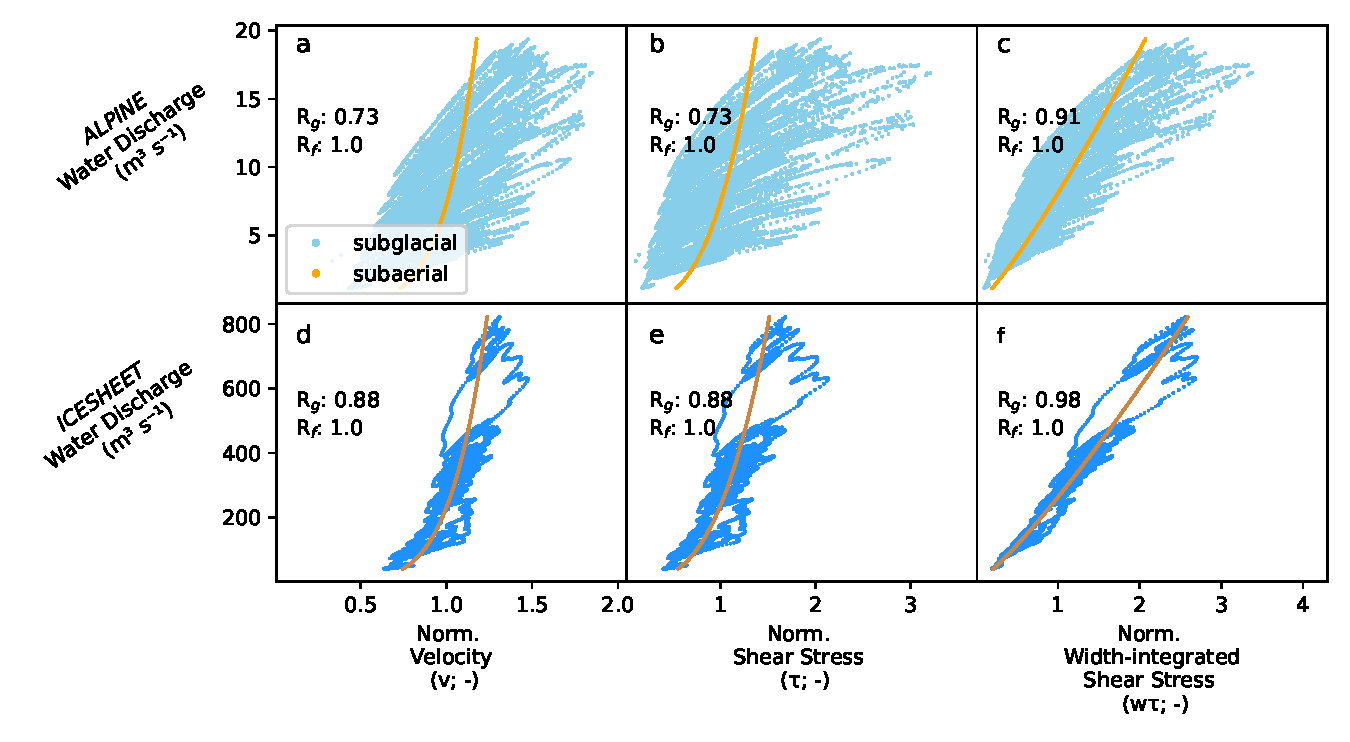
\includegraphics[width=0.7\linewidth]{Fig3.pdf}
  \caption{Standard deviation of detrended model outputs for different smoothing times with different subglacial and subaerial channel shapes and friction factors.
    Shaded areas denote the range of standard deviations from the accepted $100$ parameter combinations (Section~\ref{sect:imp}).
    Solid lines denote the mean value of standard deviations.
    Markers show smoothing periods ($15$\,\unit{min}, $1$\,\unit{hr}, $6$\,\unit{hr} $12$\,\unit{hr}, $1$\,\unit{d}, $5$\,\unit{d}, $10$\,\unit{d}, and $15$\,\unit{d}).
  }
  \label{fig:multi_run}
\end{figure}

Smaller values of $\alpha$, or a channel cross-section closer to a slot canyon, result in greater variability in velocity and shear stress (Figure~\ref{fig:params}).
In both cases, the variability of small values of $\alpha$ does not approach that of the subglacial channels.
Yet, larger values of $\alpha$ can result in greater variability in width-integrated shear stress, as greater channel width changes increase the width-integrated shear stress.
Additionally, steeper subaerial channel slopes $\nabla z_c$ result in greater variability in both shear stress and width-integrated shear stress but only approach the subglacial channel's variability in the \alpine case (Figure~\ref{fig:params}). 
We note that these parameter values span a commonly accepted range.
Therefore, we do not anticipate a scenario where variability in the subaerial system would exceed the subglacial system with these two hydrologic forcings.

Greater subglacial and subaerial friction factors $f_i$ and $f_p$ result in greater variability in the shear stress and width-integrate shear stress in both cases (Figure~\ref{fig:params}).
This result is expected given Equations~\ref{eq:tau_g} and \ref{eq:vf}.
However, more velocity variability is present in low  $f_i$ and $f_p$ values. 
Low values of $f_i$ result in slower growth rates in subglacial channels (Equations~\ref{eq:dS_dt} and \ref{eq:dh}).
As a result, water velocity, as opposed to channel growth, accommodates increases in water discharge, and velocity variability increases.
Smaller values of channel factor $\beta$, creating low and broad channels, result in more variability in width-integrated shear stress.
Here, the channel width can grow more quickly in response to water discharge increases as compared to a semi-circular channel with $\beta = \pi$ (Equation~ \ref{eq:dh}).

\begin{figure}[hbt!]
  \centering
  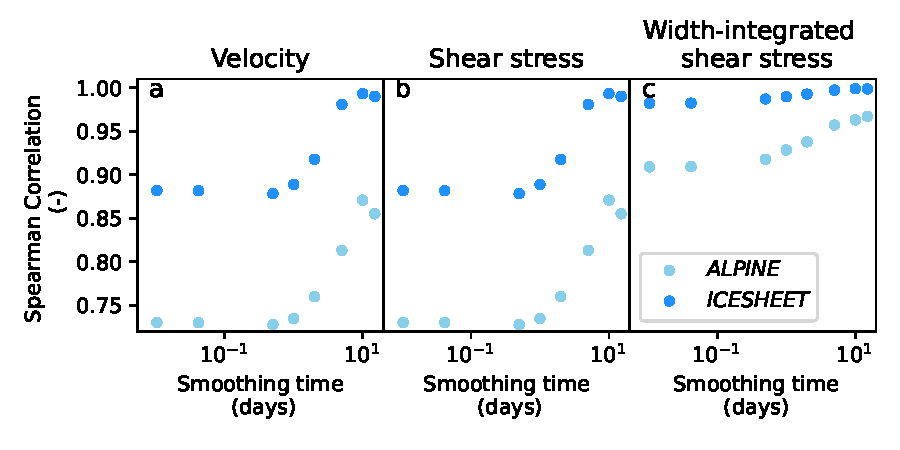
\includegraphics[width=0.7\linewidth]{Fig4.pdf}
  \caption{Parameter values compared to variability in model outputs.
    Plots on the right (orange, light blue) correspond to the \alpine{} case. Plots on the left (brown, dark blue) correspond to the \icesheet case.
    Outputs are shown using $15$ minute smoothing time. 
  }
  \label{fig:params}
\end{figure}

\FloatBarrier
\subsection{Sensitivity of sediment transport in different channel types}
\label{sect:scaling}

\begin{figure}[hbt!]
  \centering
  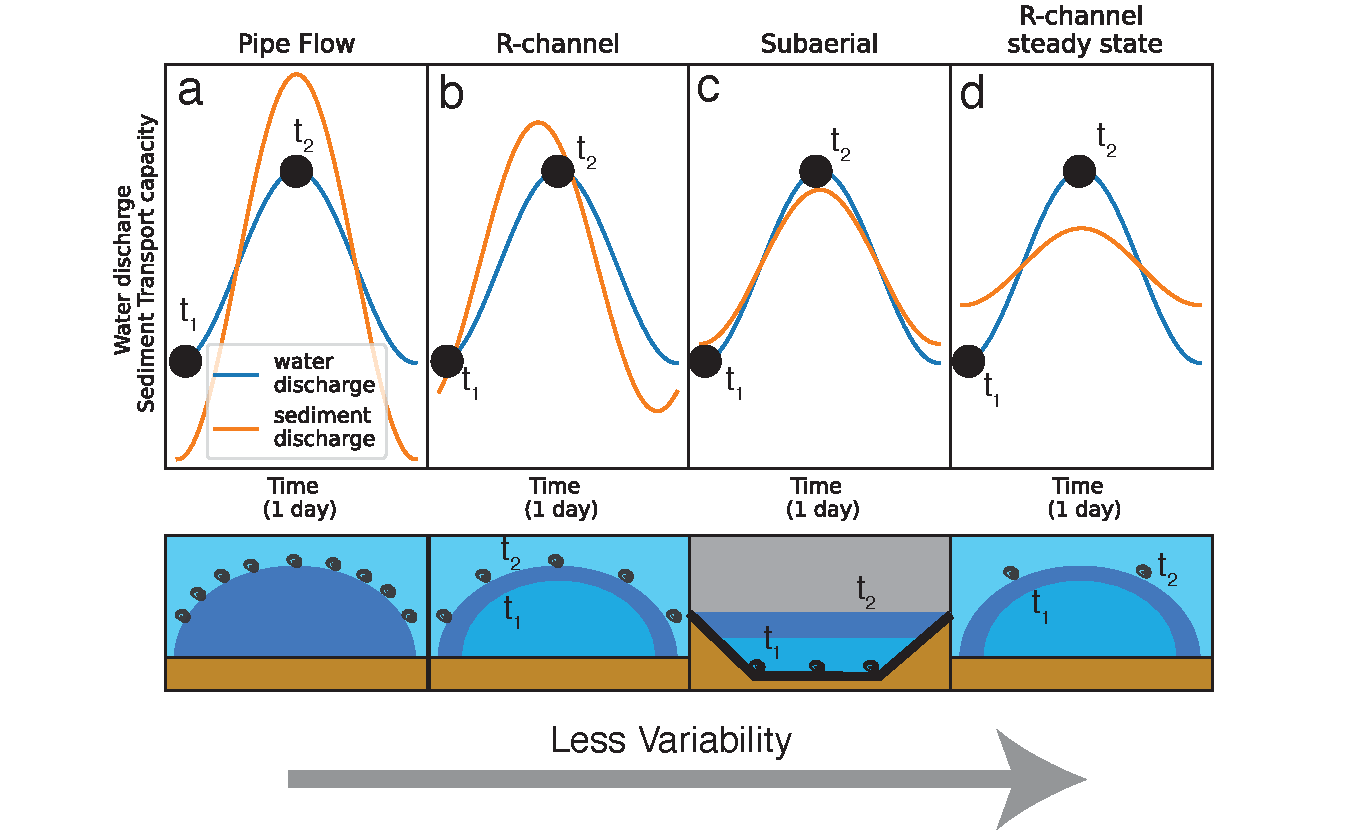
\includegraphics[width=0.7\linewidth]{Fig7.pdf}
  \caption{Response of sediment transport capacity (orange line) and channel size (bottom row) to a water discharge event (blue line) under different channel conditions.
    a) Pipe flow with fixed channel size described in Section~\ref{sect:scaling}.
    b) R-channel described in Section \ref{sect:sub_mode}.
    c) Subaerial channel described in Section~\ref{sect:fluv}.
    d) Steady-state R-channel (channel size evolves in equilibrium with water discharge) described in Section~\ref{sect:scaling}.
    Note axes are not to scale.
    $t_1$ ($t_2$) represents low (high) water discharge. 
  }
  \label{fig:chan_types}
\end{figure}

Here, we evaluate the relative sensitivity of different channel types as they scale with water discharge, channel shape, and hydraulic gradient.
These include subaerial channels (Figure~\ref{fig:chan_types} c), steady-state R-channels \citep[Figure~\ref{fig:chan_types} d]{rothlisberger1972} and pipe-flow (i.e. R-channels of fixed size that do not adjust their size to discharge conditions; Figure~\ref{fig:chan_types} a).
These formulations do not allow us to evaluate non-steady state R-channels (Section~\ref{sect:sub_mode}, Figure~\ref{fig:chan_types} b).
The sediment transport capacity is calculated with a given water discharge and hydraulic gradient for three different sediment transport capacity formulas: Meyer-Peter M\"uller  \citep[MPM; ][]{meyer1948}, Engelund and Hansen \citep[EH; ][]{engelund1967}, and Bagnold \citep{bagnold1980}; additionally width-integrated shear stress is assessed, as used as proxy for sediment transport throughout the manuscript.

Sediment discharge is given by the MPM, EH, and Bagnold formulations as
\begin{equation}
  \label{eq:Qs_eq}
  Q_s \propto w\, \tau^{3/2}, \quad Q_s \propto w\, \tau^{5/2}, \quad Q_s \propto w \left(\frac{\Omega}{w}\right)^{3/2} H^{-2/3},
\end{equation}
respectively, for conditions well above the transport onset threshold.

We use the Darcy-Weisbach equation to evaluate shear stress
\begin{equation}
  \label{eq:DW}
  \Psi \propto f\frac{Q^2}{D_h S^2},
\end{equation}
with $\Psi = \Delta h / l$ the head gradient and friction factor $f$.
The shear stress and stream power are, respectively,
\begin{equation}
  \label{eq:tau-omega}
  \tau \propto f v^2 = f \left(\frac{Q}{S}\right)^2, \quad  \Omega \propto \Psi Q.
\end{equation}
% 

As in Section~\ref{sect:fluv}, the subaerial channel is assumed to have a width $w$ much greater than its depth $H$, such that $D_h\approx 4H$, and to have a constant head gradient ($\Psi$) given by the topography.
Further, it is assumed that its width can be approximated by a relation $w \propto Q^\alpha$ (Equation~\ref{eq:wcf}) with $\alpha\in [0,1]$.
End members $\alpha=0$ or $\alpha=1$ correspond a  subaerial channels of constant width (a slot canyon) or depth (no natural equivalent), respectively.
% 
For a steady-state R-channel, it is assumed that  $\Psi$ is constant (approximated by the gradient of the \citet{shreve1972} potential) and that $S$ adjusts in steady state with $\Psi$ and $Q$.
Note that the R-channel model used above (Section~\ref{sect:sub_mode}), Equation~\ref{eq:dS_dt} calculates $\Psi$ from the time-evolving $S_g$ via the Darcy-Weisbach Equation~\ref{eq:dh} and thus no Shreve approximation is then needed.
% Conversely, pipe flow has $S$ fixed and $\Psi$ adjusts to satisfy the given $Q$.
% 
Pipe flow-like conditions occur when an R-channel is subjected to rapid discharge variations such that the channel cannot adjust its size.
In this case, it is assumed that the cross-sectional area $S$ is fixed, and $\Psi$ adjusts to the specified $Q$.
For both steady-state R-channel and pipe flow, it is assumed that $D_h \propto S^{1/2}$.

With these assumptions, the Darcy-Weisbach equation~\eqref{eq:DW} can be solved for the not-fixed quantity: $H$ for a subaerial channel, $S$ for a R-channel, and $\Psi$ for pipe-flow.
Then, using equations~\eqref{eq:tau-omega}, the shear stress and stream power can be calculated.
These results are summarised in Table~\ref{tab:eqs1}.
The results of the 12 combinations of shear stress and sediment transport capacity are presented in Table~\ref{tab:Qs} and also in Table~S1 where the fractions in the exponents are approximately given by decimal numbers for ease of comparison.

\begin{table}[hbt!]
  \caption{Relations for hydraulic variables for the three different channel types:  subaerial channels, R-channel, and pipe-flow.  Darcy-Weisbach equation is abbreviated with ``D-W'', and stream power with ``Stream p.''. }
  \small
  \label{tab:eqs1}
  \begin{tabular}{llllll}
    Channel type & Fixed & Determined via D-W
    & Additional relations & Shear stress & Stream p.\\
           & & (Equation~\ref{eq:DW})  &  &  \(\tau \propto\) & \(\Omega \propto\)\\
    \hline
    Subaerial & \(\Psi\) & \(H \propto f^{1/3}\, Q^{2/3-2\alpha/3} \, \Psi^{-1/3}\) & \makecell{\(w\,\propto Q^\alpha\) \\ \(S=wH\) \\ \(D_h\propto H\)} & \(f^{1/3} Q^{2/3-2\alpha/3}  \Psi^{2/3}\) & \(Q\, \Psi\)\\
    R-channel & \(\Psi\) & \(S\, \propto f^{2/5}\, Q^{4/5} \, \Psi^{-2/5}\) & \(D_h\propto w \propto H \propto S^{1/2}\) & \(f^{1/5} Q^{2/5} \, \Psi^{4/5}\) & \(Q\, \Psi\)\\
    Pipe & \(S\) & \(\Psi \propto f \, Q^2\, S^{-5/2}\) & \(D_h\propto w \propto H \propto S^{1/2}\) & \(f Q^2 S^{-2}\) & \(f\, Q^3 S^{-5/2}\)\\
  \end{tabular}
\end{table}

Table~\ref{tab:Qs} shows the scaling of the proxy $w\tau$ as well as $Q_s$ of the MPM, EH, and Bagnold sediment transport formulas with respect to $Q$, $\Psi$ or $S$ for the three different channel types and  $\alpha$ values.
Remarkably, the Bagnold formula has a negative exponent for $f$ in all but the pipe-flow channel type.
The total transport formula EH gives a slightly stronger dependence on all variables due to the larger exponent on $\tau$ of $\frac{5}{2}$ versus  $\frac{3}{2}$ for the MPM (Equation~\ref{eq:Qs_eq}).
Albeit, the sediment transport response in pipe flow for the Bagnold case is close to EH.
Conversely, the sediment transport proxies $w_g\,\tau_g$ and $w_f\,\tau_f$ used below scale only as $Q^2$ for pipe-flow, whereas the sediment transport capacity scales at least with $Q^3$.
The exponent for the width scaling $\alpha$ only impacts the relationship between sediment transport and water discharge in the EH relation in any meaningful way.
However, for the value of $\alpha$ around $\frac{1}{3}$ (a value appropriate for most streams), the exponent on $Q$ for EH is only slightly greater than the other transport relations.

The sediment discharge capacity in the steady state R-channel scales very similarly to the subaerial channel case for all relations and virtually identically for the $\alpha=\frac{1}{3}$ case (Table~\ref{tab:Qs}).
However, the head gradients $\Psi$ are likely higher for comparable $Q$ in an ice-sheet marginal or alpine glacier setting than in a subaerial channel \citep{alley1997}.
Thus, sediment transport capacity is likely higher in a steady-state R-channel.


\begin{table}[hbt!]
  \caption{Sediment transport proxy ($w\tau$) and rates for the three considered different transport formulas: MPM \citep{meyer1948}, EH \citep{engelund1967}, and Bagnold \citep{bagnold1980}.
  }
  \small
  \label{tab:Qs}
  \begin{tabular}{lllll}
    & Width \(\times \,\, \tau\) & MPM & EH & Bagnold\\
    & \(w\, \tau\) & \(Q_s \propto w\, \tau^{3/2}\) & \(Q_s \propto w\, \tau^{5/2}\) & \(Q_s \propto w^{-1/2}\, \Omega^{3/2} H^{-2/3}\)\\
    \hline
    Subaerial  & \(f^{1/3}\, Q^{2/3+\alpha/3}\,  \Psi^{2/3}\) & \(f^{1/2}\, Q \, \Psi\) & \(f^{5/6}\, Q^{5/3 - 2\alpha/3} \, \Psi^{5/3}\) & \(f^{-2/9}\, Q^{19/18-\alpha/18} \, \Psi^{31/18}\)\\
    R-channel & \(f^{2/5}\, Q^{4/5} \, \Psi^{3/5}\) & \(f^{1/2}\, Q \, \Psi\) & \(f^{7/10}\, Q^{7/5}\, \Psi^{9/5}\) & \(f^{-7/30}\, Q^{31/30}\, \Psi^{26/15}\)\\
    Pipe & \(f \, Q^2 \, S^{-1}\) & \(f^{3/2}\, Q^3 \, S^{-5/2}\) & \(f^{5/2}\, Q^5\, S^{-9/2}\) & \(f^{3/2} \, Q^{9/2} \, S^{-14/3}\)\\
  \end{tabular}
\end{table}

R-channels rarely operate in a steady state with variations in water discharge, especially during severe rain or melt is too short for the channel to reach a steady state (Figures~\ref{fig:model_outs} and \ref{fig:Qw_vari}).
In these cases with high water discharge variability, channels can behave more like a pipe of fixed cross-section \citep[\alpine{} case in Figure \ref{fig:Qw_vari}; e.g.][]{gimbert2016}.
Table~\ref{tab:Qs} shows that sediment transport in pipe-flow scales much more severely with discharge; the exponent on $Q$ being between $3$ and $5$, compared to the other two channel types when that exponent is at most $\frac{5}{3}$.
Thus fluctuations of discharge on short timescales (on the order of a day; Figure~\ref{fig:multi_run}) have the potential to cause conditions with very high sediment transport capacities.
These sediment transport capacities variations are of far higher magnitude than those of subaerial channels \citep[][]{alley1997}.
Note that pipe flow would cause sediment discharge capacity to covary with water discharge (Figure~\ref{fig:chan_types} a).
Covariance also occurs for steady state R-channels, but not for R-channels where channel area evolves in time (Figures~\ref{fig:Qw_vari} and \ref{fig:chan_types} b).

\FloatBarrier
\section{Discussion}

\subsection{Increased variability in  sediment transport capacity in subglacial systems}
\label{sect:dis_qsc}

The greater variations in shear stress in subglacial channels presented here may actually cause even greater variations in sediment transport capacity in subglacial channels than presented above  (Figure~\ref{fig:multi_run}).
In sediment transport capacity relationships, such as in \citet{meyer1948} or \citet{engelund1967}, shear stress is scaled to the power of $\frac{3}{2}$ or $\frac{5}{2}$, respectively (e.g. Section~\ref{sect:scaling}).
The exponent greater than $1$ magnifies sediment discharge variability beyond the variable sediment transport parameters described above (Figure~\ref{fig:multi_run}; Table~\ref{tab:Qs}).

Greater variations in subglacial sediment transport capacity could cause a supply-limited regime at many glaciers \citep{alley1997}.
In subglacial systems, sediment's critical shear stress, or threshold at which sediment mobilization occurs, can be reached more frequently and across many water discharges, compared to subaerial systems (Figure~\ref{fig:Qw_vari}).
This result suggests sediment export here is especially sensitive to observed changes in water discharge variability \citep{lane2019b}.
Sediment exhaustion through repeatedly crossing the mobilization threshold may explain the stronger dependence of sediment discharge from the Greenland Ice Sheet on basal shear stress, a proxy for bedrock erosion, rather than glacier melt \citep{overeem2017}.
The same process could also result in sediment discharge's strong dependence on sediment production from sliding in many cases \citep{herman2015,koppes2015}.

While transport-limited states at glaciers are likely rare \citep[e.g.][]{alley1997}, abundant sediment could persist underneath some glaciers, potentially creating a transport-limited regime \citep[e.g.][]{walter2014,stevens2022,delaney2022}.
At these glaciers, the great variability in subglacial sediment transport capacity may make it difficult to link sediment discharge to hydrology, especially when peak events occur \citep{cowan1988,delaney2018,lu2022}.
The results here suggest that different channel sizes with the same hydrology forcing can result in very different sediment transport capacities, making it challenging to establish the effects of individual extreme precipitation or melt events.


Catchments with reduced water discharge variability may experience yet less variability in sediment transport capacity, shown by the \alpine{} and \icesheet{} model outputs.
Indeed, the more decoupled and sporadic relationship between model outputs and water discharge in \alpine{} results from the relatively larger discharge variations on sub-daily to weekly timescales (Figure~\ref{fig:Qw_vari}).
This occurs as the subglacial channel's size evolves slowly compared to the variations in water discharge (Figure~\ref{fig:chan_types} b).
High water discharge variability in \alpine{} may cause width integrated shear stress to approach $Q^{2}$ in assuming pipe-flow conditions where the water discharge varies largely compared to channel size \citep[Figure~\ref{fig:chan_types}; Section \ref{sect:scaling}; c.f.][]{alley1997}.
Conversely, the reduced relative variability in water discharge in \icesheet{} and stronger correlation between width-integrated shear stress may result in the subglacial channel's size being closer to equilibrium from the smaller variations in water discharge (Figure~\ref{fig:chan_types} d).
In this case, the exponent on water discharge for shear stress is likely substantially less than $w\tau \propto Q^2$, but greater than $w \tau \propto Q^{\frac{4}{5}}$ that occurs in a steady-state R-channel (see Section \ref{sect:scaling}).
As a result, there is a stronger relationship between subglacial model outputs and water discharge in \icesheet{} (Figure~\ref{fig:Qw_vari}) and less variability model outputs in the \icesheet case (Figure~\ref{fig:multi_run}).

\subsection{Interpreting sediment transport records from glacierized catchments with respect to water discharge}

A sporadic relationship between subglacial sediment transport capacities and water discharge occurs due to hysteresis in subglacial channel size (Figure~\ref{fig:Qw_vari}).
This characteristic limits the use of water discharge as an indicator of sediment discharge capacity in these systems.
As a result, characteristics such as bankfull or effective water discharge that link geomorphic work to hydro-climatic conditions could have limited meaning in evaluating subglacial sediment transport \citep{wolman1960,lenzi2006}.
A glacier's sediment transport capacity is impacted by the ice thickness controlling the channel closure rate and the glacier's surface slope, in addition to water discharge and sediment size \citep[Figure~\ref{fig:multi_run}, Section~\ref{sect:sub_mode}; ][]{rothlisberger1972,gimbert2016,stevens2022,walder1994}.
This multitude of processes lies in contrast to many subaerial channels, where transport capacity typically responds to water discharge, sediment size, channel shape,  and hydraulic gradient.
The latter of these parameters can remain relatively stable over the years or longer \citep[Section~\ref{sect:fluv}; e.g.][]{tucker1997}.
Strong correlations between water discharge and sediment export in glacier systems could indicate other processes, such as increased sediment access \citep{zhang2022}.
Furthermore, the observed correlation between water discharge and sediment discharge far downstream likely represents subaerial transport processes, especially with respect to bedload \citep{mancini2023}.

The co-varying relationship between sediment discharge capacity and water discharge in subaerial conditions could be noticeable $\sim20$\,\unit{km} downstream of the Leverett site.
A strong correlation persists between sediment plume size and the Watson River's water discharge into the Kangerlussuaq fjord \citep[Figure~\ref{fig:chan_types}\,c; ][]{chu2009,mcgrath2010}.
In contrast, in marine-terminating glacier catchments, a less consistent relationship may occur between water discharge or melt extent and sediment plume size \citep{chu2012,tedstone2012}.
Here, ocean water pressurizes subglacial channels at the ice front \citep[e.g.][]{how2017}, so the observed reduced correlation could result from the inconsistent relationship between subglacial sediment transport capacity and water discharge (Figures~\ref{fig:Qw_vari} and \ref{fig:chan_types}\,b).

Water discharge measurements at less than daily timescales could severely limit subglacial sediment transport models in capturing specific events.
The decreased model output variability beyond $1$--$5$ days of smoothing could result in water discharge being in equilibrium with the subglacial channel when they are in fact not (Figure~\ref{fig:multi_run}).
Over this period, water discharge variations could lead to a stronger relationship with sediment discharge capacity (Figure~\ref{fig:chan_types} d and Section ~\ref{sect:scaling}).
Particularly, if water discharge evolves slowly with respect to the subglacial channel size, then it will covary with sediment transport capacity (Figure~\ref{fig:chan_types} d).
Such a strong relationship would not represent the impact of actual shorter-term fluctuations in water discharge.

Clockwise hysteresis loops between sediment concentration and water discharge suggest that sediment availability is reduced over the event scale \citep[][]{williams1989}.
These loops are often observed in glacierized catchments and used to suggest that access to subglacial sediment has been limited \citep[e.g.][]{collins1979,willis1996,richards2003,stott2007,delaney2018}.
Results here suggest that clockwise hysteresis could also be expected in transport-limited regimes in many subglacial environments.
Here, the smaller channel size on the rising limb would result in greater sediment transport capacity and sediment mobilization (Figure~\ref{fig:chan_types} b).
A larger channel size would reduce sediment transport capacity for an equivalent water discharge on the falling limb, creating clockwise hysteresis. 

\subsection{Experiment limitations}

Several aspects of the models and experiment design make the comparison of the subaerial and subglaical systems difficult. 
The lumped nature of the models means that they operate independently of the upstream drainage network.
Additionally, we omit analysis of suspended sediment discharge records due to their dependence on sediment supply in capturing variations in sediment discharge, in addition to sediment transport capacity \citep[e.g.][]{delaney2019}.
In reality, processes such as sediment access are usually important in controlling sediment export in glacierized catchments \citep[e.g.][]{herman2015,vergara2022}.
Furthermore, meltwater can be distributed to flow through several adjacent conduits impacting the sediment transport capacity in each \citep[e.g.][]{werder2013,hewitt2019,delaney2023}.
The lumped models used here isolate the relationship between water discharge and sediment transport capacity in subglacial and subaerial systems. 
However, they neglect more complex, yet important, spatially distributed processes.

Different hydraulic gradients control the velocity and sediment transport capacity in the subglacial and subaerial cases (Section~\ref{sect:sub_mode}~and~\ref{sect:fluv}). 
The subglacial one is generally much steeper \citep{alley1997}.
This results in the shear stresses and width-integrated shear stresses across the channel bed that controls sediment transport capacity being much greater in subglacial channels (Figure~\ref{fig:model_outs}).
The parameters' range tested in Section~\ref{sect:ensemble} covers a likely span of viable shear stresses in both subglacial and subaerial channels.
The greater sediment transport capacity in the subglacial channels implies that sediment grain size underneath subglacial channels is likely larger than subaerial counterparts.
Note, however, that the water velocities are similar in both channel types.

The channel width and size variations in subglacial channels presented here also occur in subaerial channels in response to water discharge \citep{phillips2016}, likely over decadal timescales or in response to individual extreme events \citep[e.g.][]{slater2013,dean2013}.
These timescales are likely considerably longer than the continuous changes to the subglacial channel's response time of days.
Furthermore, observations from subaerial systems can show a co-varying relationship between water discharge and sediment transport in time \citep[e.g.][]{schmidt2006,pitlick2021}.
Even so, if channel width changes occur in subaerial channels, then the values of $\alpha$ in Equation~\ref{eq:wcf} could change in time.
$\alpha$ must be less than $1$, and even this would cause the exponent on $Q$ in the  $w_g\,\tau_{g}$ relationships to remain substantially below that of pipeflow (Section ~\ref{sect:scaling}, Table\,\ref{tab:eqs1} and \ref{tab:Qs})).

Width-integrated shear stress is examined in the two numerical experiments as it does not have a dependence on grain size, unlike sediment transport relationships \citep[][Section \ref{sect:scaling}]{meyer1948}.
This makes comparison between the two systems simpler. 
Preferential transport of smaller sediment clasts and the input of upstream sediment impact sediment transport capacity as grain size evolves \citep[e.g.][]{gomez1983}.
These processes are only beginning to be evaluated underneath glaciers \citep{aitken2024}, but can be important in subaerial systems.
Subglacial sorting processes could be an additional source of variability in sediment export from glaciers with respect to water discharge, especially for bedload transport.

\conclusions

The sediment transport capacity of both subglacial and subaerial channels is driven by its width and the shear stress exerted by the flowing water, which is proportional to flow velocity squared.
Subaerial channels immediately alter both their width and water velocity in response to changing water discharge.
In contrast, pressurized subglacial channels largely accommodate rapidly changing water discharge by altering water velocity, while their size only responds to changes in discharge over longer timescales, typically, several days.
Thus, sediment transport capacity is more sensitive to changes in water discharge in subglacial channels compared to subaerial ones.

The manuscript's first objective is to establish if water discharge covaries with subglacial sediment transport capacity.
In subglacial channels, the timing of peak sediment discharge capacity occurs before peak water discharge during a discharge event, due to evolving channel size.
In subaerial channels, the timing of peak sediment discharge capacity and water discharge coincide.
Results here suggest that, even in a transport-limited subglacial system, an incoherent relationship between water and subglacial sediment discharge could be expected in most channels.
This incoherent relationship presents a challenge in linking hydro-climatic conditions or events to sediment export from glaciers.
Water discharge and sediment transport capacity covariance could be possible when water discharge varies at a slower rate than subglacial channel size.
In natural environments, this appears to rarely be the case.

The manuscript's second objective aims to evaluate the relative variability in sediment transport capacity between subglacial and subaerial channels.
Results demonstrate that sediment transport capacity variability is higher in pressurized subglacial channels that are out of equilibrium with water discharge.
Increased variability occurs even in environments where the water discharge has relatively small diurnal variations in the \icesheet case.
Yet, elevated variability is especially strong with greater water discharge variations in the \alpine case.
Further evaluation is needed to establish the role of high variability in sediment transport capacity in evaluating hydro-climatic signals from sediment records.
Greater variability in sediment transport capacity may also lead to sediment exhaustion by subglacial water repeatedly crossing the mobilization threshold across a range of water discharges. 

Few observations of the subglacial environment hinder our ability to quantify processes such as
the shape of subglacial channels and the response time of subglacial channels to water discharge variations.
The poor constraints on subglacial sediment size and sorting processes make it difficult to link shear stress to sediment discharge capacity.
Further quantifying these processes will help to better inform the response of sediment discharge capacity to water discharge forcing in subglacial environments.

This study calls for the explicit consideration of evolving channel size when examining the relationship between sediment transport and hydro-climatic conditions from glacierized catchments, especially ones with high water discharge variability.

\codedataavailability{
  Code, with links to the data, can be found at \url{https://bitbucket.org/IanDelaney/xsection/src/master/}.
  Data from Leverett glacier have been previously published in \citet{tedstone2013}.
  Data from Fieschergletscher have been previously published in \citet{delaney2024}.
  The code will be uploaded to a permanent repository, with FAIR principles pending acceptance of the paper.}

\authorcontribution{
  I.D. designed the study, developed, and implemented the model and experiments, and wrote the manuscript.
  A.J.T. helped interpret findings from Leverett Glacier and guided experiment design.
  M.A.W. and D.F. provided data from Fieschergletscher and contributed to analysis.
  All authors provided key inputs in writing and editing the manuscript.} %% this section is mandatory

\competinginterests{The authors declare no competing interests.} %% This section is mandatory even if you declare that no competing interests are present

\begin{acknowledgements}
  SNSF Project No. $\mathrm{PZ00P2}$\_$202024$ provided  funding for I. Delaney.
  A. Tedstone acknowledges funding from the European Research Council, award $818994$ -- CASSANDRA.
  G. King and M. J. Gevers provided useful comments on a previous version of this manuscript.
  We benefited from fruitful discussions with J. Irving.
  We thank two reviewers for constructive and critical reviews on a previous version of the manuscript.
\end{acknowledgements}
%\newpage
%\appendix

% \appendixtables   %% needs to be added in front of appendix tables


% \appendixfigures  %% needs to be added in front of appendix figures

% 

%% Please add \clearpage between each table and/or figure. Further guidelines on figures and tables can be found below.




\bibliographystyle{copernicus}
\bibliography{Paperlib.bib}


%% REFERENCES

%% The reference list is compiled as follows:

% \begin{thebibliography}{}

% \bibitem[AUTHOR(YEAR)]{LABEL1}
%   REFERENCE 1

% \bibitem[AUTHOR(YEAR)]{LABEL2}
%   REFERENCE 2

% \end{thebibliography}

%% Since the Copernicus LaTeX package includes the BibTeX style file copernicus.bst,
%% authors experienced with BibTeX only have to include the following two lines:
%% 
%% 
%% \bibliography{example.bib}
%% 
%% URLs and DOIs can be entered in your BibTeX file as:
%% 
%% URL = {http://www.xyz.org/~jones/idx_g.htm}
%% DOI = {10.5194/xyz}


%% LITERATURE CITATIONS
%% 
%% command                        & example result
%% \citet{jones90}|               & Jones et al. (1990)
%% \citep{jones90}|               & (Jones et al., 1990)
%% \citep{jones90,jones93}|       & (Jones et al., 1990, 1993)
%% \citep[p.~32]{jones90}|        & (Jones et al., 1990, p.~32)
%% \citep[e.g.,][]{jones90}|      & (e.g., Jones et al., 1990)
%% \citep[e.g.,][p.~32]{jones90}| & (e.g., Jones et al., 1990, p.~32)
%% \citeauthor{jones90}|          & Jones et al.
%% \citeyear{jones90}|            & 1990



%% FIGURES

%% When figures and tables are placed at the end of the MS (article in one-column style), please add \clearpage
%% between bibliography and first table and/or figure as well as between each table and/or figure.

% The figure files should be labelled correctly with Arabic numerals (e.g. fig01.jpg, fig02.png).


%% ONE-COLUMN FIGURES

%% f
% \begin{figure}[t]
%   \includegraphics[width=8.3cm]{FILE NAME}
%   \caption{TEXT}
% \end{figure}
% 
%%% TWO-COLUMN FIGURES
% 
%% f
% \begin{figure*}[t]
%   \includegraphics[width=12cm]{FILE NAME}
%   \caption{TEXT}
% \end{figure*}
% 
% 
%%% TABLES
%%% 
%%% The different columns must be seperated with a & command and should
%%% end with \\ to identify the column brake.
% 
%%% ONE-COLUMN TABLE
% 
%% t
% \begin{table}[t]
%   \caption{TEXT}
%   \begin{tabular}{column = lcr}
      %       \tophline
      %       
      %       \middlehline
      %       
      %       \bottomhline
      %     \end{tabular}
      %       \belowtable{} % Table Footnotes
      %       \end{table}
      %       
      %%%       TWO-COLUMN TABLE
      %       
      %%       t
      %       \begin{table*}[t]
      %       \caption{TEXT}
      %       \begin{tabular}{column = lcr}
      %       \tophline
      %       
      %       \middlehline
      %       
      %       \bottomhline
      %     \end{tabular}
      %       \belowtable{} % Table Footnotes
      %       \end{table*}
      %       
      %%%       LANDSCAPE TABLE
      %       
      %%       t
      %       \begin{sidewaystable*}[t]
      %       \caption{TEXT}
      %       \begin{tabular}{column = lcr}
      %       \tophline
      %       
      %       \middlehline
      %       
      %       \bottomhline
      %     \end{tabular}
      %       \belowtable{} % Table Footnotes
      %       \end{sidewaystable*}
      %       
      %       
      %%%       MATHEMATICAL EXPRESSIONS
      %       
      %%%       All papers typeset by Copernicus Publications follow the math typesetting regulations
      %%%       given by the IUPAC Green Book (IUPAC: Quantities, Units and Symbols in Physical Chemistry,
      %%%       2nd Edn., Blackwell Science, available at: http://old.iupac.org/publications/books/gbook/green_book_2ed.pdf, 1993).
      %%%       
      %%%       Physical quantities/variables are typeset in italic font (t for time, T for Temperature)
      %%%       Indices which are not defined are typeset in italic font (x, y, z, a, b, c)
      %%%       Items/objects which are defined are typeset in roman font (Car A, Car B)
      %%%       Descriptions/specifications which are defined by itself are typeset in roman font (abs, rel, ref, tot, net, ice)
      %%%       Abbreviations from 2 letters are typeset in roman font (RH, LAI)
      %%%       Vectors are identified in bold italic font using \vec{x}
      %%%       Matrices are identified in bold roman font
      %%%       Multiplication signs are typeset using the LaTeX commands \times (for vector products, grids, and exponential notations) or \cdot
      %%%       The character * should not be applied as mutliplication sign
      %       
      %       
      %%%       EQUATIONS
      %       
      %%%       Single-row equation
      %       
      %       \begin{equation}
      %       
      %       \end{equation}
      %       
      %%%       Multiline equation
      %       
      %       \begin{align}
      %       & 3 + 5 = 8\\
      %               & 3 + 5 = 8\\
      %               & 3 + 5 = 8
                        %     \end{align}
                        %                         
                        %                         
                        %%%     MATRICES
                        %                         
                        %                         \begin{matrix}
                        %                         x & y & z\\
      %       x & y & z\\
      %       x & y & z\\
      %       \end{matrix}
      %       
      %       
      %%%       ALGORITHM
      %       
      %       \begin{algorithm}
      %       \caption{...}
      %       \label{a1}
      %       \begin{algorithmic}
      %       ...
      %       \end{algorithmic}
      %       \end{algorithm}
      %       
      %       
      %%%       CHEMICAL FORMULAS AND REACTIONS
      %       
      %%%       For formulas embedded in the text, please use \chem{}
      %       
      %%%       The reaction environment creates labels including the letter R, i.e. (R1), (R2), etc.
      %       
      %       \begin{reaction}
      %%%         \rightarrow should be used for normal (one-way) chemical reactions
      %%%         \rightleftharpoons should be used for equilibria
      %%%         \leftrightarrow should be used for resonance structures
      %       \end{reaction}
      %       
      %       
      %%%       PHYSICAL UNITS
      %%%       
      %%%       Please use \unit{} and apply the exponential notation


\end{document}


      %       \ian{comeback here}
      %       For sufficiently short periods, channel width and wetted area are fixed in the subglacial system (akin to pipe flow) so that the response of width-integrated shear stress is $w_g\, \tau_{g}\, \propto\,  Q^{2}$ \citep[Table\,~\ref{tab:Qs}; ][]{alley1997}.

      %       R\"othlisberger channels in steady state with water discharge (i.e. channel sizes evolves at a faster rate than water discharge), the width-integrated shear stress response to water discharge is $ w_g\,\tau_{g}\, \propto\,  Q^{\sim\frac{4}{5}}$ (Table\,~\ref{tab:Qs}).
      %       This relationship suggests that when discharge varies more slowly than channel shape subglacial channels have less variable sediment transport capacity than subaerial ones.
      %       Yet, subglacial channels rarely operate in a steady state \citep{gimbert2016}.
      %       However, the reduced variability in the  \icesheet{} case compared to the \alpine{} one suggests that it is closer to an equilibrium state (Figure~\ref{fig:Qw_vari}).
      %       \ian{comeback here}
      %       The channel width and size variations in subglacial channels presented here also occur in subaerial channels in response to water discharge \citep{phillips2016}, likely over decadal timescales or in response to individual extreme events \citep{slater2013,dean2013}.
      %       These timescales are considerably longer than the continuous changes to the subglacial channel's response time of days.
      %       Even so, if channel width changes occur in subaerial channels, then the values of $\alpha$ in Equation~\ref{eq:wcf} could change in time.
      %       $\alpha$ must be less than $1$, and even this would cause the exponent on $Q$ in the  $w_g\,\tau_{g}$ relationships to remain substantially below that of pipeflow (see Sections \ref{sect:scaling}, Table~\ref{tab:Qs}, Figure~\ref{fig:multi_run}).

With even smaller water discharge variations, the subglacial sediment transport capacity may behave similarly to the subaerial system.
Note that in pipe flow conditions, maximum sediment transport would coincide with peak water discharge, unlike the evolving channel size alters the timing (Figure \ref{fig:model_outs} and \ref{fig:Qw_vari}).


When sediment availability processes are considered, a glacier's sediment discharge record also represent sediment availability and bedrock erosion from water pressure variations and sliding  \citep[e.g. ][]{iverson2012,herman2015,delaney2023}.
The greater amount of in variability of subglacial sediment evacuation can make it difficult to isolate the drivers of sediment export with respect to hydrological and glaciological conditions \citep{delaney2024}.
